\chapter[Avaliação e Interpretação]{AVALIAÇÃO E INTERPRETAÇÃO}

Este capítulo corresponde à Etapa 6 do processo KDD, na qual o conhecimento sobre os dados e sobre os modelos é sintetizado. Como lembra a proposta do trabalho, os dados são compreendidos por meio dos modelos.

\section{ESPECTRO COMPLETO DE SUPERVISÃO}

A Figura \ref{fig:espectro} e a Tabela \ref{tab:espectro} reúnem, em uma mesma escala, o desempenho obtido com 0\% de rótulos (K-Médias com mapeamento húngaro), com taxas intermediárias (melhor \textit{baseline} e melhor semi-supervisionado de cada taxa) e com 100\% de rótulos (classificadores supervisionados treinados com todo o treino).

\begin{figure}[htbp]
    \centering
    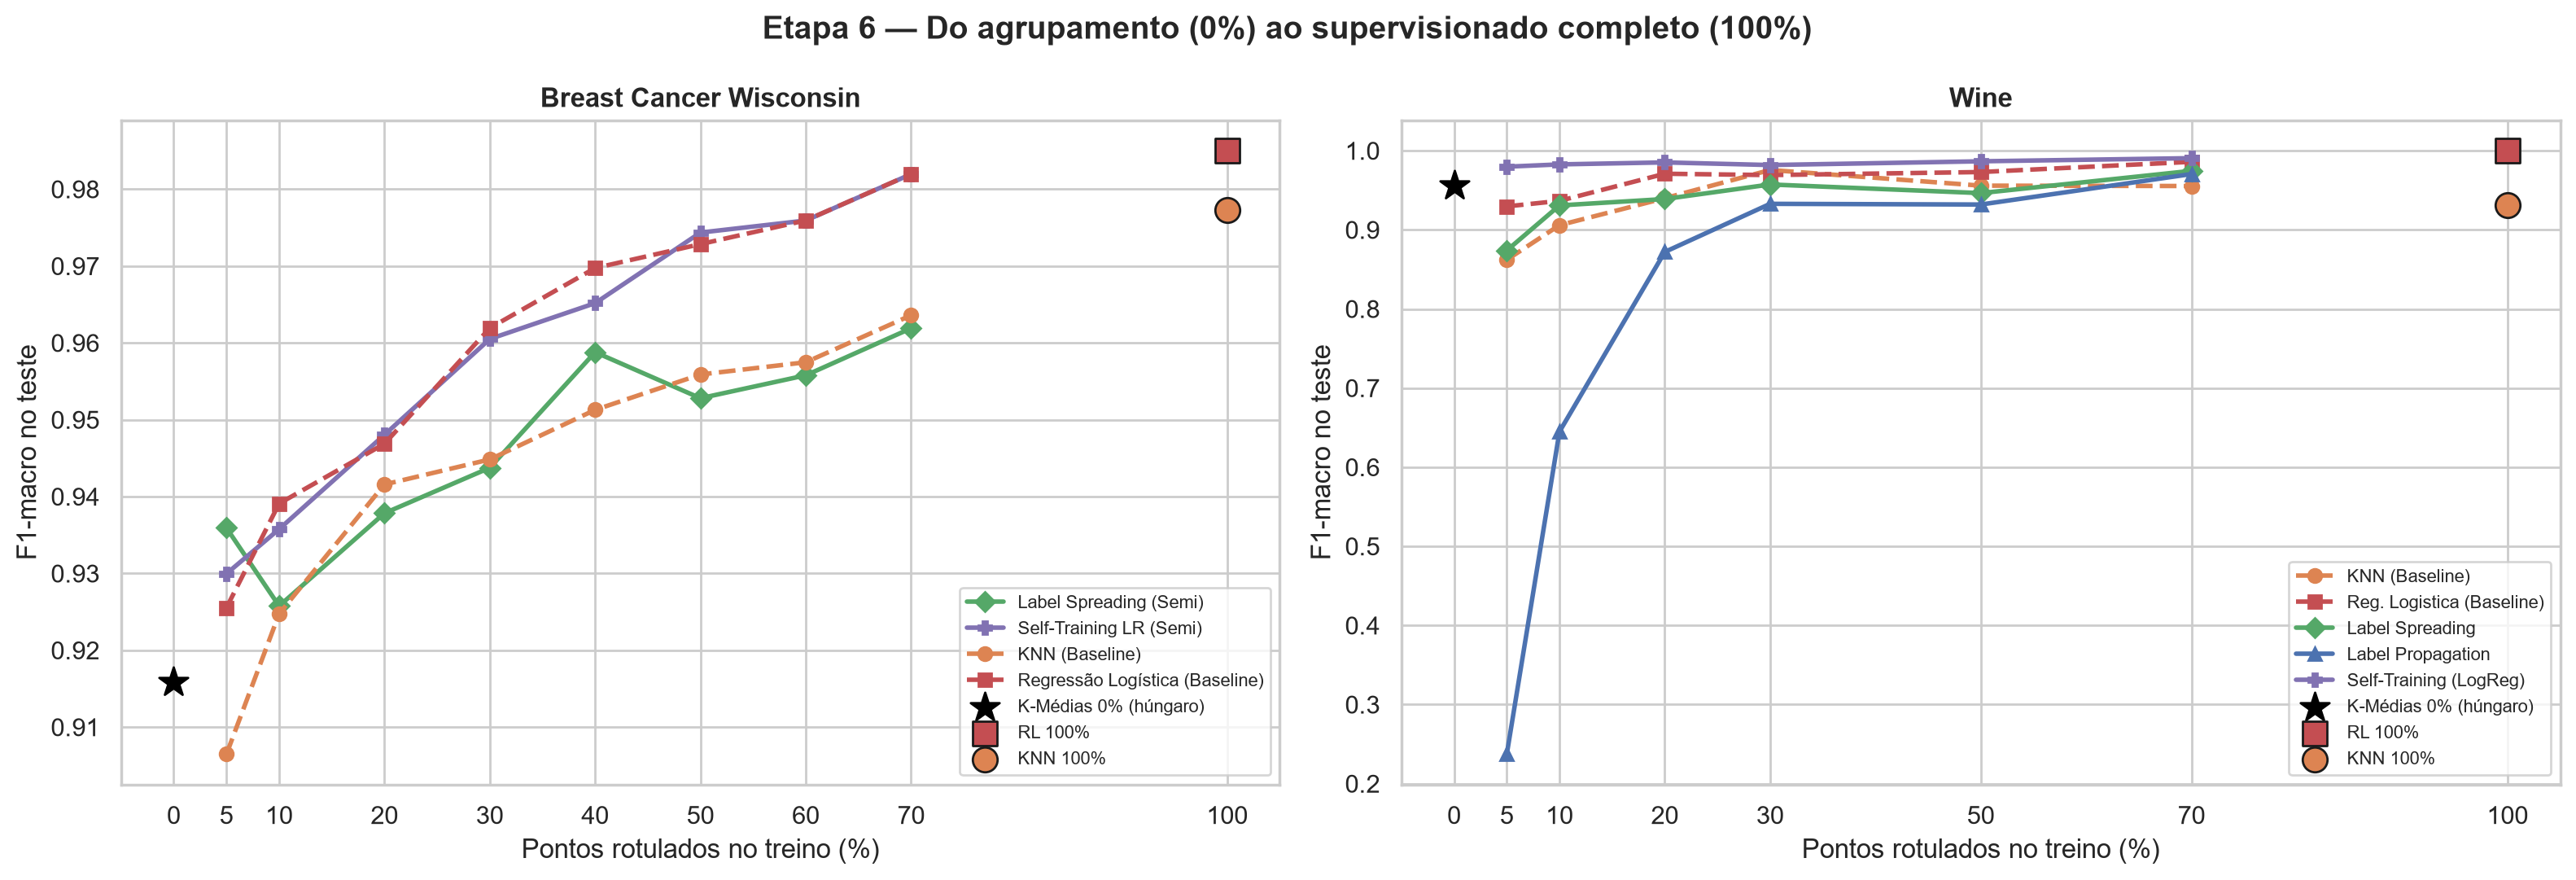
\includegraphics[width=\textwidth, keepaspectratio]{figuras/E6_espectro_supervisao.png}
    \caption{F1-macro no teste ao longo de todo o espectro de supervisão, do agrupamento (0\%) ao supervisionado completo (100\%).}
    \label{fig:espectro}
\end{figure}

\begin{table}[htbp]
\centering
\caption{F1-macro no teste ao longo do espectro de supervisão.}
\label{tab:espectro}
\footnotesize
\begin{tabular}{lccccccc}
\toprule
 & \textbf{0\%} & \multicolumn{2}{c}{\textbf{5\%}} & \multicolumn{2}{c}{\textbf{70\%}} & \multicolumn{2}{c}{\textbf{100\%}} \\
\cmidrule(lr){3-4} \cmidrule(lr){5-6} \cmidrule(lr){7-8}
\textbf{Base} & \textbf{K-Médias} & \textbf{Baseline} & \textbf{Semi} & \textbf{Baseline} & \textbf{Semi} & \textbf{RL} & \textbf{KNN} \\
\midrule
Breast Cancer & 0,916 & 0,926 & 0,936 & 0,982 & 0,982 & 0,985 & 0,977 \\
Wine & 0,956 & 0,930 & 0,980 & 0,986 & 0,991 & 1,000 & 0,931 \\
\bottomrule
\end{tabular}
\end{table}

Dois aspectos se destacam. Primeiro, no Wine, o K-Médias sem nenhum rótulo (0,956) supera a Regressão Logística treinada com 5\% dos rótulos (0,930), e o \textit{Self-Training} com 5\% (0,980) já se aproxima do desempenho supervisionado completo. Segundo, no Breast Cancer, o ganho entre 0\% e 100\% é obtido de forma gradual, e o melhor método em cada taxa alterna entre semi-supervisionados e a Regressão Logística.

\section{O QUE OS MODELOS REVELAM SOBRE OS ATRIBUTOS}

Treinada com 100\% dos rótulos no espaço padronizado, a Regressão Logística tem coeficientes comparáveis entre si: o sinal indica a direção do efeito, e a magnitude, a importância \textit{condicional} (dados os demais atributos).

No \textbf{Breast Cancer}, os atributos com maiores coeficientes (\texttt{worst texture}, \texttt{radius error}, \texttt{worst symmetry}, \texttt{worst concave points} e \texttt{area error}) diferem do ranking univariado da ANOVA (correlação de Spearman de 0,589 entre os rankings). Isso é consequência da forte multicolinearidade observada na Etapa 3: a Regressão Logística distribui o peso entre as variáveis redundantes de tamanho, de modo que a importância condicional difere da marginal. Os \textbf{pontos côncavos} aparecem nos dois rankings e são o marcador mais robusto de malignidade.

No \textbf{Wine}, há maior concordância entre os rankings (Spearman de 0,670): \texttt{proline}, \texttt{flavanoids}, \texttt{alcohol} e \texttt{color\_intensity} estão entre os cinco primeiros nos dois casos.

\section{ANÁLISE DE ERROS}

Para cada amostra de teste, foi calculada a taxa de erro considerando todos os modelos, taxas e repetições do experimento semi-supervisionado. A Figura \ref{fig:erros_bc} mostra o resultado para o Breast Cancer.

\begin{figure}[htbp]
    \centering
    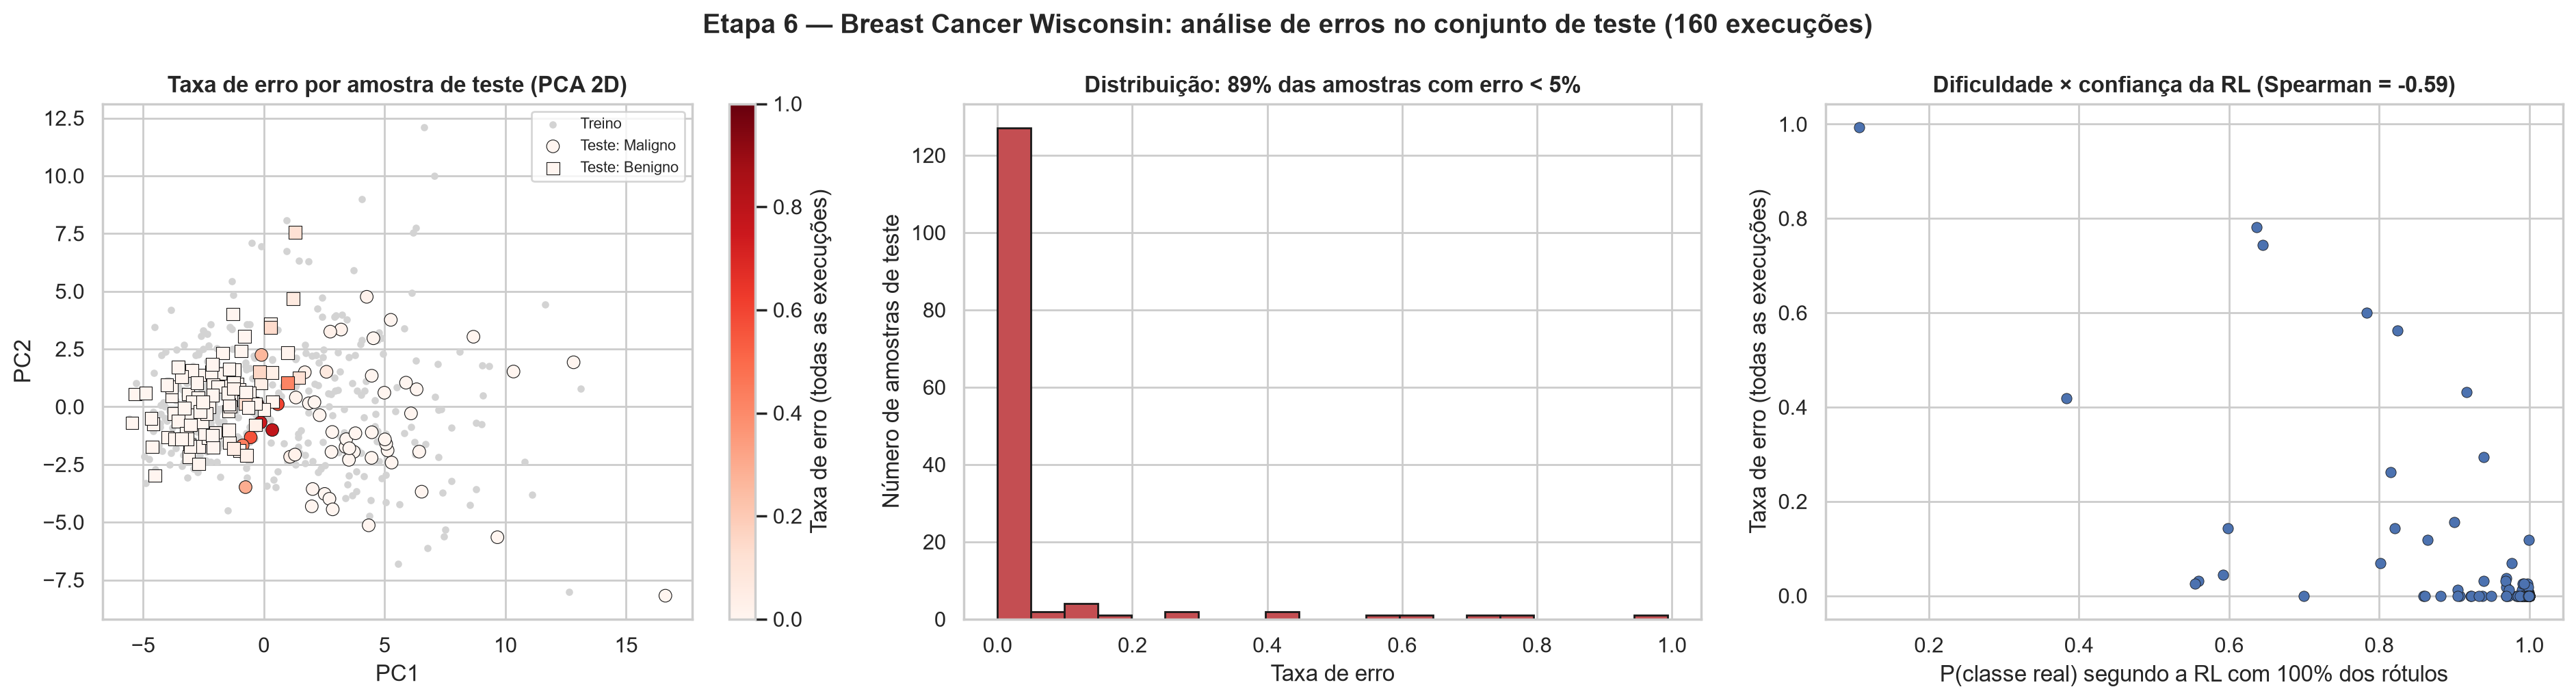
\includegraphics[width=\textwidth, keepaspectratio]{figuras/E6_breast_cancer_analise_erros.png}
    \caption{Breast Cancer Wisconsin: taxa de erro por amostra de teste, considerando as 160 execuções do experimento, e sua relação com a probabilidade atribuída à classe real pela Regressão Logística com 100\% dos rótulos.}
    \label{fig:erros_bc}
\end{figure}

No Breast Cancer, 88,8\% das amostras de teste quase nunca são classificadas incorretamente (taxa de erro menor que 5\%). As seis amostras mais difíceis são todas \textbf{malignas classificadas como benignas}, ou seja, falsos negativos, o erro mais grave em um contexto de triagem. Elas ficam na fronteira entre as classes no PCA. Uma delas é classificada incorretamente em 99,4\% das execuções, e até a Regressão Logística com 100\% dos rótulos lhe atribui probabilidade de malignidade de apenas 0,107. Trata-se de um caso atípico, possivelmente com rótulo ruidoso, o que não é possível verificar com os dados disponíveis. No Wine, a proporção de amostras ``fáceis'' é menor (57,8\%), porque o colapso do \textit{Label Propagation} com poucos rótulos produz muitos erros em várias execuções.

\section{REVISÃO DAS HIPÓTESES}

Como o processo KDD não é linear, a mineração pode contradizer as hipóteses iniciais. A Tabela \ref{tab:veredito} aplica os critérios objetivos definidos na Etapa 1.

\begin{table}[htbp]
\centering
\caption{Revisão das hipóteses formuladas na Etapa 1.}
\label{tab:veredito}
\footnotesize
\begin{tabular}{p{0.6cm} p{2.4cm} p{8.4cm} p{2.6cm}}
\toprule
\textbf{\#} & \textbf{Base} & \textbf{Evidência} & \textbf{Resultado} \\
\midrule
H1 & Breast Cancer & F1 da Regressão Logística com 100\% dos rótulos = 0,985 & Confirmada \\
\addlinespace
H2 & Breast Cancer & 5\%: \textit{Label Spreading} $-$ RL = $+$0,010 (vence 4/5; $p = 0{,}125$). 10\%: \textit{Self-Training} $-$ RL = $-$0,003 (vence 1/5; $p = 0{,}500$) & 5\%: inconclusiva; 10\%: refutada \\
\addlinespace
H2 & Wine & 5\%: \textit{Self-Training} $-$ RL = $+$0,050 (vence 8/10; $p = 0{,}008$). 10\%: $+$0,046 (vence 9/10; $p = 0{,}004$) & Confirmada \\
\addlinespace
H3 & Breast Cancer & $\Delta F1$ (melhor semi $-$ melhor \textit{baseline}): 5\% = $+$0,010; 70\% = 0,000 & Confirmada \\
\addlinespace
H3 & Wine & $\Delta F1$: 5\% = $+$0,050; 70\% = $+$0,005 & Confirmada \\
\addlinespace
H4 & Ambas & ARI do K-Médias: Wine = 0,908; Breast Cancer = 0,672 & Confirmada \\
\addlinespace
H5 & Breast Cancer & ARI: DBSCAN = 0,025; K-Médias = 0,672 & Confirmada \\
\addlinespace
H5 & Wine & ARI: DBSCAN = 0,602; K-Médias = 0,908 & Confirmada \\
\addlinespace
H6 & Breast Cancer & F1 do KNN: completo = 0,962; PCA 2D = 0,932 (96,9\%) & Confirmada \\
\addlinespace
H6 & Wine & F1 do KNN: completo = 0,963; PCA 2D = 0,978 (101,6\%) & Confirmada \\
\bottomrule
\end{tabular}
\end{table}

\section{SÍNTESE}

\textbf{O benefício do semi-supervisionado depende da estrutura dos dados, e não só da escassez de rótulos.} No Wine, as cultivares formam grupos compactos (ARI do K-Médias de 0,908), a hipótese de \textit{cluster} vale e os pontos não rotulados ajudam muito: com 5\% de rótulos, o \textit{Self-Training} supera a Regressão Logística em 0,050 de F1, com significância estatística. No Breast Cancer, a fronteira entre as classes é essencialmente linear (H1), e um modelo supervisionado simples com o viés indutivo adequado é tão bom quanto as alternativas semi-supervisionadas. A vantagem observada a 5\% diminui com mais rótulos (H3), mas não é estatisticamente sustentada.

\textbf{O agrupamento funciona como diagnóstico.} O caso com 0\% de rótulos antecipou onde o semi-supervisionado ajudaria: quando o K-Médias já recupera as classes (Wine), os dados não rotulados agregam informação; quando não recupera (Breast Cancer), não agregam.

\textbf{Sobre os modelos.} O \textit{Self-Training} com Regressão Logística foi o melhor semi-supervisionado em média nas duas bases, porque herda o viés linear da Regressão Logística e acrescenta pseudo-rótulos de boa qualidade, desde que o limiar de confiança seja adequado. Os métodos de grafo (\textit{Label Propagation} e \textit{Label Spreading}) mostraram-se muito sensíveis aos hiperparâmetros $\gamma$, $\alpha$ e \texttt{n\_neighbors}, que foram fixados \textit{a priori}. Ajustá-los exigiria dados rotulados de validação, justamente o recurso escasso nesse cenário. As diferenças entre a avaliação indutiva (teste) e a transdutiva (pontos não rotulados do treino) foram pequenas, no máximo cerca de 0,05 em F1, e não indicaram sobreajuste sistemático aos pontos não rotulados.

\textbf{Revisão do processo.} O resultado inconclusivo no Breast Cancer leva de volta à Etapa 1: a hipótese de que o semi-supervisionado ajuda quando há poucos rótulos precisa ser condicionada à estrutura de agrupamento dos dados e testada com repetições suficientes. Uma nova iteração do processo poderia (a) aumentar o número de repetições no Breast Cancer, (b) ajustar $\gamma$ e $\alpha$ dos métodos de grafo por validação cruzada sobre os poucos rótulos disponíveis e (c) ajustar o limiar de decisão para reduzir os falsos negativos.

\textbf{Limitações.} Foi usada uma única partição treino/teste. No Wine, o teste tem 45 amostras, de modo que um erro equivale a 2,2 pontos de acurácia. Os p-valores do teste de Wilcoxon são indicativos, pois todas as repetições usam o mesmo conjunto de teste. Por fim, os protocolos das duas bases diferem entre si (taxas, repetições, modelos e hiperparâmetros), e por isso as comparações entre as bases são qualitativas.

\section{PÓS-PROCESSAMENTO}

A Etapa 7, opcional, consistiu na exportação de todas as figuras e tabelas de métricas para uso neste relatório e na apresentação, e na formulação das seguintes recomendações práticas:

\begin{itemize}
    \item \textbf{Breast Cancer:} em um cenário com poucos laudos, uma Regressão Logística sobre atributos padronizados, treinada apenas com os casos rotulados, é a opção mais simples e mais fácil de auditar, e as alternativas semi-supervisionadas não mostraram vantagem estatisticamente sustentada sobre ela. Como os erros residuais são falsos negativos, o limiar de decisão deve ser escolhido priorizando a sensibilidade para a classe maligna. O modelo é um apoio à triagem e não substitui o diagnóstico do patologista.
    \item \textbf{Wine:} com apenas 7 vinhos rotulados, o \textit{Self-Training} com Regressão Logística já atinge F1 de 0,98 usando os demais vinhos sem rótulo, o que reduz o custo de rotulagem por análise especializada. O limiar de confiança deve ser escolhido com cuidado, pois limiares altos anulam o ganho.
    \item \textbf{Reprodutibilidade:} sementes fixas, versões das bibliotecas registradas e todas as métricas exportadas em arquivos CSV.
\end{itemize}
